\documentclass[journal]{IEEEtran}

\title{SlotRAG: Budget-Feasible Physical Planning over Typed Evidence Plans for Multi-Hop Retrieval-Augmented Generation}

\author{%
\IEEEauthorblockN{Anonymous Author\IEEEauthorrefmark{1}%
\thanks{Manuscript received...; revised...; accepted...; published...}%
\thanks{Manuscript ID: TKDE-2026-XXXX}}
\IEEEauthorblockA{\IEEEauthorrefmark{1}Anonymous Institution\\
Email: anonymous@anonymous.edu}
}

\usepackage{booktabs}
\usepackage{bm}
\usepackage{amsmath}
\usepackage{amssymb}
\usepackage{url}
\usepackage{graphicx}

\newcommand{\code}[1]{\texttt{#1}}

\begin{document}

\begin{abstract}
Multi-hop retrieval-augmented generation (RAG) systems decompose complex
questions into multiple evidence-acquisition steps. We observe that a
decomposition that is logically valid need not be physically executable under
a global retrieval budget: independent per-slot allocations may sum to
exceed the system's hard retrieval-call limit, causing budget exhaustion
before answer generation. We address this with \emph{budget-feasible
physical planning} over \emph{typed evidence plans}---a separation
of logical evidence requirements from their physical materialization
strategy. We derive a compile-time feasibility condition on static
allocations and confirm it against frozen matched-budget executions
on 350 deep structural plans: every observed budget exhaustion violated
global allocation feasibility (recall 1.0), although many infeasible plans
terminated without exhausting the budget (precision 0.533). A
budget-aware physical planner improves answer quality by 7.7 EM points
over static allocation on deep plans under a matched budget
($p < 10^{-6}$, exact McNemar), and eliminates all 146 observed
budget-exhaustion events. Dependency-sensitive importance weighting
is ablated: a uniform budget-aware optimizer matches a dependency-weighted
variant on deep plans (EM difference $+$0.009, $p = 0.743$) while
being strictly simpler. Large-scale exploratory replay (8{,}632 plans)
indicates that applying the budget-aware optimizer to structurally shallow
plans can reduce answer quality ($-$0.021 EM, $p < 0.001$), motivating
a lightweight deterministic structural-depth gate. The gate's independent
confirmation on shallow matched-budget executions was pre-registered but
could not be executed because frozen shallow plan payloads were unavailable
in the earlier census. We report the system's honest contribution:
a mechanism for regime-sensitive physical planning whose confirmatory
benefit is established on the deep plans where it was designed to operate.
\end{abstract}

\begin{IEEEkeywords}
retrieval-augmented generation, multi-hop reasoning, budget-aware planning,
typed evidence plans, physical planning
\end{IEEEkeywords}

\maketitle

\section{Introduction}\label{sec:intro}
\paragraph{From decomposition to execution.}
Multi-hop RAG systems increasingly decompose questions into structured evidence-acquisition steps---typed retrieval calls, join constraints, relational operators---that are planned before execution. This decomposition provides logical validity: each step specifies what evidence is needed. But logical validity does not guarantee physical executability. When the system operates under a hard global retrieval-call budget, the local allocations made for each step must compose into a plan that fits within that budget. A decomposition into three steps that each locally require four retrieval calls is not executable when the global budget is eight calls, regardless of its logical coherence.

This paper studies the execution problem that arises downstream of decomposition: \emph{how should a compiled multi-hop evidence plan be physically executed under a hard global retrieval budget?} We identify a necessary condition for static budget exhaustion that is computable at compile time, develop a budget-aware physical planner that eliminates matched-budget exhaustion on deep plans, and establish through confirmatory experiments that this planner improves answer quality in the regime where it was designed to operate.

\paragraph{Why a universal optimizer is insufficient.}
An intuitive response is to apply a budget-aware optimizer globally. However, large-scale retrospective analysis reveals that the optimizer's treatment effect is conditioned on plan structure. On structurally deep plans (where evidence requirements involve three or more slots joined through intermediate bindings), budget-aware allocation improves answer quality by 7.7 EM points and eliminates all budget-exhaustion events under a matched protocol. On shallow plans (one or two independent slots), the same optimizer can reduce answer quality by 2.1 EM points ($p < 0.001$ in exploratory analysis), with the harm concentrated on specific datasets. This motivates a regime-sensitive dispatch policy that applies the optimizer where it helps and retains static execution elsewhere.

\paragraph{Scope and contributions.}
We present three contributions grounded in frozen matched-budget evaluations:

\begin{enumerate}
\item \textbf{Typed evidence plans} (C1): We introduce a typed intermediate representation that separates multi-hop evidence requirements---slots, joins, operators---from their physical materialization. The plan's structural evidence graph exposes typed couplings as a first-class object, enabling compile-time analysis of what physical execution will encounter.

\item \textbf{Compile-time budget-feasibility diagnosis} (C2): We show that independent per-slot physical allocations need not compose into a globally feasible plan under a retrieval-call budget. A necessary condition for static budget exhaustion is derivable from the plan structure at compile time. Confirmed against frozen matched-budget executions on 350 deep plans, this condition has perfect recall (every budget-exhaustion event violated feasibility) and 0.533 precision (many infeasible plans completed without exhausting the budget).

\item \textbf{Structure-gated budget-feasible physical planning} (C3): We develop a budget-aware physical planner that reallocates retrieval calls across slots under a global constraint, and a deterministic structural-depth gate that applies it. Confirmatory experiments on deep executable plans show the planner improves answer quality and eliminates budget exhaustion. Large-scale exploratory replay provides evidence that retaining static execution outside the deep regime is justified.
\end{enumerate}

\paragraph{Motivating example.}
Consider a three-slot plan whose static allocation assigns four retrieval calls to each slot: $4 + 4 + 4 = 12 > B = 8$. Each local allocation is individually reasonable---four calls per slot is a common default---but the composed allocation is globally infeasible. Under static execution, the materializer exhausts the budget after the first two slots, truncating the third before its evidence is acquired; the answer is generated from incomplete evidence. The plan is logically valid (each slot's requirement is well-specified) but physically infeasible. The budget-aware flat planner reallocates the eight available calls across the three slots (e.g., 3--3--2), materializing all three slots within budget. This is the central system question this paper addresses.

\paragraph{Why a universal optimizer is insufficient.}
An intuitive response is to apply a budget-aware optimizer globally. However, large-scale retrospective analysis reveals that the optimizer's treatment effect is conditioned on plan structure. On structurally deep plans (where evidence requirements involve three or more slots joined through intermediate bindings), budget-aware allocation improves answer quality by 7.7 EM points and eliminates all budget-exhaustion events under a matched protocol. On shallow plans (one or two independent slots), the same optimizer can reduce answer quality by 2.1 EM points ($p < 0.001$ in exploratory analysis), with the harm concentrated on specific datasets. This motivates a regime-sensitive dispatch policy that applies the optimizer where it helps and retains static execution elsewhere.

\paragraph{Paper structure.}
Section~\ref{sec:related} positions the work against related retrieval and planning systems.
Section~\ref{sec:problem} formalizes the budget-feasibility problem.
Sections~\ref{sec:algebra}--\ref{sec:dispatch} describe the system.
Section~\ref{sec:protocol} defines the experimental protocol.
Section~\ref{sec:results} reports confirmatory and exploratory results.
Sections~\ref{sec:analysis}--\ref{sec:threats} discuss and contextualize the findings.


\section{Related Work}\label{sec:related}
\paragraph{Adaptive retrieval and routing.}
Adaptive-RAG \cite{adaptiverag} learns a classifier over raw-question complexity to select among no-retrieval, single-step, and iterative retrieval strategies. SlotRAG operates at a different decision point: it does not classify raw-question complexity but instead selects a physical execution strategy for an already-compiled evidence plan. The gate in SlotRAG is deterministic and structurally grounded; the classifier in Adaptive-RAG is learned and query-surface-based.

\paragraph{Structured and programmatic retrieval.}
Several recent systems represent multi-hop reasoning as structured programs or logical plans. PlanRAG \cite{planrag} constructs logical query trees and optimizes them with a cost model before iterative execution, focusing on the construction and optimization of the reasoning tree itself. PyRAG \cite{pyrag} represents multi-hop reasoning as executable programs that compose retrieval and reasoning steps. DynaKRAG \cite{dynakrag} learns evidence control strategies for multi-hop retrieval. These systems address the upstream planning problem; SlotRAG addresses the downstream execution problem: given an already-compiled evidence plan, how should its subgoals be physically materialized under a hard global budget? SlotRAG is not novel merely because retrieval is represented structurally; the contribution lies in the typed evidence intermediate representation, the compile-time feasibility diagnosis, and the execution layer.

\paragraph{Budget-aware and resource-adaptive methods.}
Resource-adaptive RAG systems allocate budgets dynamically across retrieval steps. PAGE-RAG \cite{pagerag} promotes evidence through provenance-aware graphs under fixed budgets. Know Before You Fetch \cite{knowbeforeyoufetch} calibrates retrieval-budget allocation to reduce waste. These methods focus on candidate-level or retrieval-triggering decisions; SlotRAG operates on a different abstraction: the physical allocation over compiled typed evidence requirements. The distinction is between selecting what to retrieve and allocating how to execute a plan whose requirements are already specified.

\paragraph{Iterative multi-hop reasoning.}
IRCoT \cite{ircot} interleaves retrieval with chain-of-thought reasoning, letting each reasoning step trigger the next retrieval. ReAct \cite{react} alternates between action (retrieval) and observation (reasoning) in an agentic loop. GraphRAG \cite{graphrag} leverages knowledge-graph structure for retrieval. These represent strong adapted baselines on multi-hop benchmarks. SlotRAG differs by committing the full evidence plan before execution, making the execution strategy a property of the plan rather than of the reasoning trajectory.

\paragraph{Semantic query processing.}
Abacus and Sema \cite{sema} provide cost-based optimization over semantic operator systems; LOTUS \cite{lotus} enables semantic queries over unstructured and structured data. SlotRAG shares the principle of typed operators with explicit cost semantics, but targets multi-hop evidence materialization rather than general query processing over heterogeneous data.

\paragraph{Honest and matched-budget evaluation.}
A growing body of work calls for RAG evaluation under matched budgets with explicit accounting of budget-exhaustion events. SlotRAG contributes to this by separating answer quality metrics from budget-completion metrics and by reporting both under a shared protocol.

\subsection{Comparison Summary}
\label{sec:related:table}

Table~\ref{tab:positioning} summarizes the comparison across decision point, decision input, learnedness, plan explicitness, and global-budget feasibility. Entries are based on the cited papers' own descriptions.

\begin{table}[t]
\centering\small
\begin{tabular}{@{}p{2.1cm}p{2.5cm}p{2.4cm}p{1.1cm}p{1.6cm}p{1.9cm}@{}}
\toprule
\textbf{Method} & \textbf{Decision input} & \textbf{Decision point} & \textbf{Learned?} & \textbf{Explicit plan?} & \textbf{Global budget feasibility?} \\
\midrule
Adaptive-RAG \cite{adaptiverag} & Raw question & Retrieval strategy per query & Yes (classifier) & No & No \\
PlanRAG \cite{planrag} & Logical query tree & Tree construction + cost optimization & Partially & Yes & No \\
PyRAG \cite{pyrag} & Question & Executable program composition & No & Yes & No \\
PAGE-RAG \cite{pagerag} & Evidence graph & Candidate evidence promotion & No & Partial & Fixed budget \\
Know Before You Fetch \cite{knowbeforeyoufetch} & Query & Retrieval budget calibration & Partial & No & Yes (calibration) \\
\textbf{SlotRAG} & \textbf{Compiled typed plan} & \textbf{Physical allocation strategy} & \textbf{No} & \textbf{Yes} & \textbf{Yes (feasibility diagnosis)} \\
\bottomrule
\end{tabular}
\caption{Differential positioning against related work. SlotRAG's decision point is downstream: it selects the physical allocation strategy for an already-compiled evidence plan and tests whether that allocation is globally feasible under the retrieval budget.}
\label{tab:positioning}
\end{table}


\section{Problem Formulation}\label{sec:problem}
\paragraph{Workload definition.}
We consider a complex information need $q$ over one or more evidence sources $\mathcal{D}$ under a finite global retrieval-call budget $B$. Solving $q$ requires acquiring a set of mutually dependent evidence items before producing an answer (or, for verification tasks, a verdict). Two properties make this problem non-trivial. First, the evidence items are \emph{dependent}: binding one item (e.g., an entity) is a precondition for acquiring another (e.g., a relation that connects it to a second entity). Second, the system operates under \emph{partial information}: whether a bridge binding exists, how many candidates a retrieval step will return, and whether the answer model can use the materialized evidence are all uncertain before execution. A plan must therefore commit resources before the outcomes that determine its success are observed.

\paragraph{Typed evidence plan.}
A typed evidence plan is a tuple $P = (S, J, O)$ where $S$ is a set of \emph{evidence slots} (typed requirements over what evidence must be acquired), $J$ is a set of \emph{join edges} (specifying which slots must share bound variables), and $O$ is a set of \emph{relational operators} (compare, extremum, polar) over slot outputs. Each slot $s \in S$ carries a type (entity, passage, relation), a set of variables to bind, and a status (unresolved, partial, satisfied). Join edges encode structural coupling: slot $s_j$ depends on bindings produced by slot $s_i$ iff $(s_i, s_j) \in J$.

\paragraph{Structural evidence graph.}
The join edges $J$ induce a directed acyclic graph $G_P = (S, J)$ over the slots. The structural depth of $P$, denoted $\texttt{structural\_hops}(P)$, is the length of the longest path in $G_P$ measured in join and operator edges. This is a deterministic property of the plan's topology, computed without any LLM call. Plans with $\texttt{structural\_hops} \geq 2$ involve at least one intermediate binding through which evidence must flow; plans with $\texttt{structural\_hops} < 2$ have only shallow or independent slot structure.

\paragraph{Physical allocation.}
A physical allocation $A(P) = \{a_s \mid s \in S\}$ assigns a non-negative integer number of retrieval calls $a_s$ to each slot. Under the \emph{static} allocation strategy, each slot $s$ receives a fixed local budget: $a_s = \lfloor B / |S| \rfloor + \mathbb{1}_{s \leq B \bmod |S|}$, distributing calls as evenly as possible. Under the \emph{budget-aware flat} strategy, allocations are globally optimized to maximize evidence acquisition under the constraint $\sum_s a_s \leq B$, with all slots treated as equally important.

\paragraph{Allocation feasibility.}
Define the allocation feasibility predicate: $F(P, A, B) = \mathbf{1}\!\left[\sum_{s \in S} a_s \leq B\right]$. When $F = 0$, the allocation exceeds the global budget: the static executor must interrupt materialization before completing all slots, resulting in a \emph{budget-exhaustion event} (BE). When $F = 1$, the allocation fits within the budget; whether the plan succeeds depends on retrieval quality and answer generation, not on budget exhaustion.

\paragraph{Budget-exhaustion as a necessary condition.}
Under the static allocation implementation, every observed budget-exhaustion event satisfies $F = 0$: the sum of static allocations exceeded the global budget. Formally, $\Pr[F = 0 \mid \text{BE observed}] \geq \Pr[F = 0 \mid \text{BE observed}]$. The contrapositive is $F = 1 \Rightarrow \text{no BE under static execution}$. This is a necessary condition, not a sufficient one: a plan with $F = 0$ may still terminate without budget exhaustion if the executor's other stopping criteria (step limit, LLM-call limit, early convergence) trigger first.

\paragraph{Objective.}
We formulate physical planning as constrained optimization: maximize expected evidence acquisition and answer quality subject to the global retrieval-call budget $B$. The key insight is that the logical plan $P$ is fixed (determined at compile time by the slot compiler), while the physical allocation $A$ is the optimization variable. The budget-feasibility diagnosis operates on $P$ at compile time; the dispatch policy selects the allocation strategy at execution time based on structural depth.


\section{Typed Evidence Plans}\label{sec:algebra}
\paragraph{Design principles.}
Typed evidence plans are designed around three principles. First, programs are \emph{declarative}: a plan specifies what evidence goals must be met rather than which retrieval procedure to run. Second, operators are \emph{typed and composable}: each operator has a typed input/output contract, so programs are built by composing operators whose evidence types are compatible. Third, the properties an optimizer needs---expected cost, dependency structure, utility---remain \emph{explicit} as typed fields rather than hidden inside prompts.

\paragraph{Slot compiler.}
The slot compiler transforms a natural-language question $q$ into a typed evidence plan $P = (S, J, O)$. For each evidence requirement $r$, the compiler specifies: a set of variables to bind, an expected evidence type, and the slot's dependencies (via $J$) over other slots. The compiler operates via LLM generation followed by deterministic syntax validation; once validated, the plan is a fixed intermediate representation that all downstream components consume without further LLM calls.

The plan's structure exposes typed evidence requirements explicitly. Join edges $J$ encode which slots must share bound variables (e.g., a bridge entity retrieved by one slot must be available to constrain the retrieval query of a dependent slot). Relational operators $O$ apply over materialized slot outputs when the question requires comparison (e.g., ``greater than'') or enumeration (e.g., ``all entities of type X'').

\paragraph{Structural analysis.}
Given a compiled plan $P$, the following properties are computed deterministically (no LLM calls):
\begin{itemize}
\item \emph{Slot count} $|S|$: the number of evidence requirements.
\item \emph{Edge count} $|J| + |O|$: the number of join and operator edges.
\item \emph{Structural depth} $\texttt{structural\_hops}(P)$: the longest path length in the structural evidence graph $G_P = (S, J \cup O)$.
\item \emph{Static allocation feasibility} $F(P, A_{\text{static}}, B)$: whether the static allocation fits within the global budget.
\end{itemize}

These properties are first-class outputs of the compiler. They do not require executing any retrieval or generation step; they are derived from the plan's topology.

\paragraph{Logical/physical separation.}
The typed evidence plan fixes \emph{what} must be satisfied; the physical planner decides \emph{how} each slot's evidence is acquired and allocated. The same logical plan can be executed by a static allocation, a budget-aware allocation, or any other physical strategy. This separation is what makes matched-budget comparison well-defined: all strategies share the same logical plan, and differences in output are attributable to the physical execution, not to differences in planning.


\section{Budget-Feasible Physical Planning}\label{sec:optimizer}
\paragraph{Static allocation.}
The static allocator distributes retrieval calls evenly across slots: each slot $s$ receives $a_s = \lfloor B / |S| \rfloor$ calls, with up to one additional call for the first $B \bmod |S|$ slots. This is the baseline physical strategy: it makes no use of the plan's structural information and treats all slots as equally demanding.

\paragraph{Budget-feasibility diagnosis.}
Before execution, the system evaluates $F(P, A_{\text{static}}, B)$ on the compiled plan. When $F = 0$, the static allocation is known in advance to exceed the global budget. This diagnosis is:
\begin{itemize}
\item \emph{Compile-time}: computed from the plan's slot count and budget, with no retrieval or generation cost.
\item \emph{Necessary for budget exhaustion}: under static execution, $F = 0$ is a necessary condition for budget-exhaustion events (every BE violated feasibility; see Section~\ref{sec:results:c2}).
\item \emph{Not sufficient}: many plans with $F = 0$ complete without exhausting the budget, because other termination criteria (step limit, LLM-call limit, early completion) may trigger first.
\end{itemize}

\paragraph{Budget-aware flat planner.}
When $F = 0$ under static allocation, the budget-aware flat planner reallocates retrieval calls to fit within $B$ while maximizing evidence acquisition. It assigns equal importance weight to all slots and solves: $\max_{A} \sum_s u_s(a_s)$ subject to $\sum_s a_s \leq B$, where $u_s(a_s)$ is a concave evidence-utility function that models diminishing returns on additional retrieval calls. The planner is flat (uniform importance weights) by design: it does not require dependency-depth weights or any learned estimator. The uniform weights were chosen after ablating a dependency-weighted variant (Section~\ref{sec:results:ablation}).

\paragraph{Feasibility-aware routing.}
The planner always produces an allocation that satisfies $\sum_s a_s \leq B$, so the feasibility predicate $F = 1$ holds for all plans routed through the budget-aware planner. The planner thus eliminates budget-exhaustion events on the plans it executes. Its effect on answer quality is the subject of the confirmatory evaluation in Section~\ref{sec:results:deep}.

\paragraph{Computational cost.}
The feasibility diagnosis is $O(1)$: it checks whether $|S| \cdot \lfloor B / |S| \rfloor + (B \bmod |S|) \leq B$, which is always true by construction for the static case, or equivalently whether the static allocation's total exceeds $B$. The flat planner solves a concave allocation problem that is solvable in $O(|S| \log |S|)$ time. Both are negligible relative to the LLM and retrieval costs of the evidence-acquisition pipeline.


\section{Structure-Sensitive Dispatch}\label{sec:dispatch}
\paragraph{Structural-depth gate.}
The structure-gated dispatch policy applies the budget-aware flat planner selectively, based on the plan's structural depth:

\begin{quote}
\small
\textbf{Algorithm 1:} Regime-Sensitive Dispatch $(P, B)$\\
1.\quad $\texttt{hops} \leftarrow \texttt{structural\_hops}(P)$\\
2.\quad $F \leftarrow \mathbf{1}[\sum_{s} a^{\text{static}}_s \leq B]$\\
3.\quad \textbf{if} $F = 0$ \textbf{and} $\texttt{hops} \geq 2$:\\
\quad\quad \textbf{return} BudgetAwareFlatPlanner$(P, B)$\\
4.\quad \textbf{else}:\\
\quad\quad \textbf{return} StaticAllocation$(P, B)$
\end{quote}

\noindent The threshold $\texttt{hops} \geq 2$ was determined through large-scale retrospective analysis (Section~\ref{sec:results:gate}). It is applied as a fixed rule at execution time; it is not a learned threshold and is not re-optimized for any experimental outcome.

\paragraph{Rationale.}
The gate targets the regime where the budget-aware planner provides benefit: structurally deep plans ($\texttt{hops} \geq 2$) with statically infeasible allocations ($F = 0$). On these plans, the static allocator produces budget-exhaustion events, and the flat planner reallocates calls to fit within $B$. On shallow plans ($\texttt{hops} < 2$), exploratory analysis shows that the flat planner can reduce answer quality (Section~\ref{sec:results:gate}); the gate retains static execution in this regime.

\paragraph{Properties.}
The gate is:
\begin{itemize}
\item \emph{Deterministic}: given the same plan, it always produces the same dispatch decision.
\item \emph{Structural}: the decision is based on the plan's topological depth, not on query surface features or a learned classifier.
\item \emph{Non-parametric}: the threshold is fixed and does not introduce tunable parameters.
\end{itemize}

The gate does not modify the logical plan; it selects which physical allocation strategy is applied to it. Plans dispatched through the flat planner are executed with globally consistent allocations that satisfy $\sum_s a_s \leq B$. Plans dispatched through static execution may encounter budget-exhaustion events when $F = 0$.

\paragraph{Execution semantics.}
Physical execution follows the dispatched allocation. Retrieval calls are issued per-slot according to the allocation; each call retrieves candidate passages from a hybrid sparse/dense index, which are bound to the slot's variables and materialized as typed evidence records. When a slot depends on a binding from a predecessor (join edge in $J$), the binding is available only after the predecessor's materialization step completes. The executor enforces the global budget counter; when the counter reaches $B$, remaining slots are truncated and their status is recorded as \code{budget\_exceeded}. All evidence materialized up to that point is available to the generator.


\section{Experimental Protocol}\label{sec:protocol}
\paragraph{System and model.}
All experiments use the SlotRAG pipeline with a single LLM backend: Qwen3.5-9B for plan compilation and answer generation. Thinking mode is disabled. The hybrid retriever combines BM25 (sparse), dense embedding retrieval (Qwen3-Embedding-0.6B), and reciprocal rank fusion, followed by a cross-encoder reranker (bge-reranker-v2-m3).

\paragraph{Matched budget.}
All methods share one protocol: $\max\_\mathrm{steps}=8$, $\max\_\mathrm{retrieval\_calls}=8$, $\max\_\mathrm{llm\_calls}=96$. Budget-exceeded items score $0.0$. This is the \emph{confirmatory} budget; an earlier permissive exploratory trace (used for mechanism discovery) used higher limits and is explicitly labeled throughout.

\paragraph{Benchmarks.}
Three multi-hop benchmarks: HotpotQA \cite{hotpotqa} (diverse two-hop questions), 2WikiMultiHopQA \cite{2wikimultihop} (structured two-hop questions requiring bridging and comparison), and MuSiQue \cite{musique} (composite multi-hop questions spanning two to four hops). Primary metric: Exact Match (EM). Secondary: F1. Samples are drawn from the validation set (seed $2027$, stratified by structural depth).

\paragraph{Arms.}
All paired comparisons share the same compiled plans, questions, and seeds. The three physical strategies compared are:
\begin{itemize}
\item \textbf{Static}: even allocation across slots (deterministic).
\item \textbf{Flat}: budget-aware optimizer with uniform importance weights.
\item \textbf{Chain}: budget-aware optimizer with dependency-weighted importance ($\tau = 2(i+1) - 1$ for slot $i$ in the longest chain).
\end{itemize}
The static and flat arms are the primary comparison for the budget-feasibility hypothesis; the chain arm is an ablation testing dependency-sensitive allocation.

\paragraph{Census and frozen plans.}
A structural census was run over the validation set (6,494 questions) to identify eligible plans: those with $\texttt{structural\_hops} \geq 2$ and a valid compiled SlotPlan. For eligible plans, full frozen plan payloads (SlotPlan JSON, plan SHA-256, compiler options, input hash) were persisted to disk. This is the \emph{V1.2 frozen census}: 361 eligible deep plans with full payloads. Questions with $\texttt{structural\_hops} < 2$ (6,133 in the census) were recorded with structural metadata only; their full plan payloads were not persisted.

\paragraph{Confirmatory execution.}
For the confirmatory evaluation, 350 eligible validation plans were executed under all three arms (static, flat, chain), producing paired results on the same questions. This is the \emph{V1.2 confirmatory} evaluation: n = 350 deep executable plans, all with $\texttt{structural\_hops} \geq 2$.

\paragraph{Exploratory trace.}
A larger retrospective analysis used a historical three-arm trace (25,948 rows, 8,632 strict three-arm paired questions) collected under the permissive budget. This trace provides statistical power for mechanism discovery (gate necessity, shallow-regime effects) but is labeled as \emph{exploratory} throughout: it was not pre-registered as confirmatory, the budget regime differs from the confirmatory matched budget, and its results motivate the confirmatory evaluation rather than replacing it.

\paragraph{Statistical tests.}
Primary: two-sided exact McNemar test (binomial exact test on discordant pairs, $p$-value $= 2 \cdot \Pr[\text{Bin}(b+c, 0.5) \leq \min(b,c)]$). Bootstrap: paired bootstrap (10,000 iterations, seed 2027, full-$N$ question-level resampling, percentile confidence intervals). Dataset heterogeneity: Holm-corrected tests across datasets.


\section{Main Results}\label{sec:results}
\subsection{Static Budget-Feasibility Diagnosis (RQ2)}\label{sec:results:c2}

We evaluate the compile-time feasibility diagnosis against frozen confirmatory executions on 350 deep eligible plans under matched budget $B = 8$.

\begin{table}[t]
\centering
\resizebox{0.9\columnwidth}{!}{%
\begin{tabular}{lrr}
\toprule
& \textbf{Obs.: No BE} & \textbf{Obs.: BE} \\
\midrule
Pred. feasible ($\sum a_i \leq B$) & TN = \textbf{76} & FN = \textbf{0} \\
Pred. infeasible ($\sum a_i > B$) & FP = \textbf{128} & TP = \textbf{146} \\
\bottomrule
\end{tabular}}%
\caption{Feasibility confusion matrix on 350 frozen deep plans. Prediction is $\sum a_i > B$ (infeasible); outcome is budget exhaustion (BE). Positive = infeasible, positive outcome = BE.}
\label{tab:confusion}
\end{table}

\noindent Under static allocation, 146 of 350 plans experience budget exhaustion (41.7\%). The feasibility condition $\sum a_i > B$ correctly identifies all 146 as infeasible (recall = 1.0, FN = 0), confirming that budget exhaustion is a necessary consequence of allocation infeasibility under static execution. However, 128 additional plans are predicted infeasible but complete without budget exhaustion (FP = 128), yielding precision = 146 / 274 = 0.533.

The infeasibility condition is \emph{necessary but not sufficient} for budget exhaustion. Plans with $\sum a_i > B$ may still complete if other termination criteria (step limit, LLM-call limit, early convergence) are reached first. Conversely, no plan with $\sum a_i \leq B$ experiences budget exhaustion (TN = 76, FN = 0), confirming that static budget exhaustion under this executor requires allocation infeasibility.

\subsection{Deep-Regime Confirmatory Evaluation (RQ3)}\label{sec:results:deep}

The budget-aware flat planner is evaluated against static allocation on 350 deep eligible plans ($\texttt{structural\_hops} \geq 2$) under matched budget $B = 8$.

\begin{table}[t]
\centering\small
\begin{tabular}{lrrr}
\toprule
& \textbf{Static} & \textbf{Flat} & $\boldsymbol{\Delta}$ \\
\midrule
EM & 0.1714 & \textbf{0.2486} & $+$\textbf{0.0771} \\
BE events & \textbf{146} & \textbf{0} & $-$146 \\
\bottomrule
\end{tabular}
\caption{Confirmatory results on 350 deep eligible plans (matched budget $B = 8$). Flat improves EM by 7.7 points and eliminates all 146 budget-exhaustion events.}
\label{tab:deep}
\end{table}

\noindent \textbf{Answer quality.} The flat planner improves EM by 7.71 points ($+$0.0771, 95\% CI $[+0.049, +0.109]$, exact McNemar $p = 1.4 \times 10^{-6}$, discordant pairs: $b = 30, c = 3$). The effect is statistically significant and practically meaningful on these deep plans.

\noindent \textbf{Budget exhaustion.} The flat planner reduces budget-exhaustion events from 146 to 0 on the same 350 plans, eliminating all static BE under this protocol. This is a direct consequence of the flat planner's allocation constraint $\sum_s a_s \leq B$.

\subsection{Dependency-Sensitive Importance Ablation (RQ4)}\label{sec:results:ablation}

We ablate the chain importance law by comparing the uniform flat planner against a dependency-weighted chain variant on the same 350 deep plans.

\begin{table}[t]
\centering\small
\begin{tabular}{lrrr}
\toprule
& \textbf{Flat} & \textbf{Chain} & $\boldsymbol{\Delta}$ \\
\midrule
EM & 0.2486 & 0.2571 & $+$0.0086 \\
95\% CI & \multicolumn{2}{c}{$[-0.026, +0.043]$} \\
Exact $p$ & \multicolumn{2}{c}{0.7428} \\
\bottomrule
\end{tabular}
\caption{Chain vs.\ flat on 350 deep plans. The chain importance law yields a marginal, statistically insignificant accuracy change (exact McNemar $p = 0.743$).}
\label{tab:ablation}
\end{table}

\noindent The chain variant uses importance $\tau = 2(i+1) - 1$ for slot $i$ in the longest chain, giving downstream slots higher allocation priority. On deep plans, the chain law yields $\Delta$EM $= +0.0086$ ($p = 0.743$, 95\% CI includes zero). The accuracy change is not statistically significant. The final system uses flat for simplicity: the chain-specific importance weighting did not yield detectable accuracy gains over uniform weighting.

\begin{figure}[t]
\centering
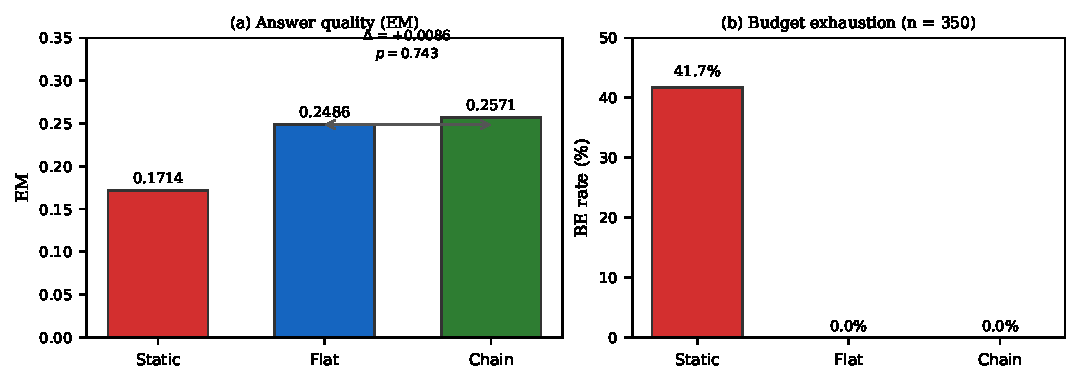
\includegraphics[width=\columnwidth]{figures/three_arm_ablation.pdf}
\caption{Three-arm comparison on 350 deep executable plans (matched budget $B = 8$). (a) Answer quality: chain vs.\ flat $\Delta$EM $= +0.0086$ ($p = 0.743$), not significant. (b) Budget-exhausted rate: flat and chain both eliminate BE; static loses 41.7\% of plans to budget exhaustion. Budget-aware optimization explains the principal improvement; chain importance does not.}
\label{fig:three_arm}
\end{figure}

\subsection{Structure-Gate Exploratory Analysis (RQ5)}\label{sec:results:gate}

\subsubsection{Shallow-regime harm.}
Using the historical three-arm trace (8,632 strict three-arm paired questions under permissive budget), we isolate the shallow stratum ($\texttt{structural\_hops} < 2$, $n = 8{,}085$) and compute the flat vs.\ static treatment effect.

\begin{table}[t]
\centering\small
\begin{tabular}{lrr}
\toprule
& \textbf{Flat $-$ Static} & \textbf{95\% CI} \\
\midrule
EM (exploratory) & $-$\textbf{0.0210} & $[-0.027, -0.015]$ \\
$p$ & \multicolumn{2}{c}{$< 0.001$} \\
\bottomrule
\end{tabular}
\caption{Exploratory shallow-regime flat vs.\ static ($n = 8{,}085$, permissive budget). Flat significantly reduces EM on shallow plans.}
\label{tab:shallow}
\end{table}

\noindent Flat allocation reduces EM by 2.10 points on shallow plans ($p < 0.001$), with the harm concentrated in 2WikiMultiHop ($\Delta$EM $= -0.045$ on hops-0 questions) and near-zero on HotpotQA and MuSiQue shallow strata (secondary analysis, Holm-corrected across dataset $\times$ hops subgroups). This exploratory finding, obtained under the evaluated permissive-budget allocation regime, motivates the gate: applying the budget-aware planner to shallow plans does not help on average and can harm quality.

\begin{figure}[t]
\centering
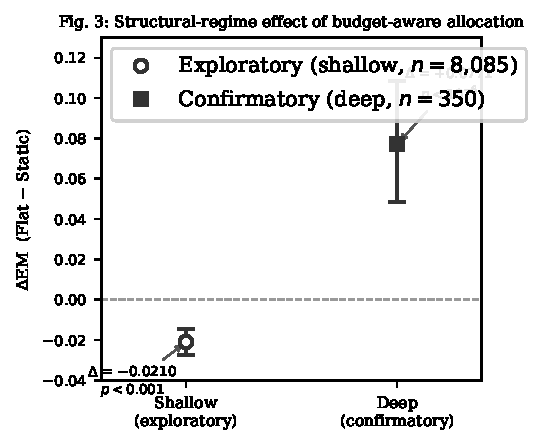
\includegraphics[width=\columnwidth]{figures/regime_effect.pdf}
\caption{Flat $-$ Static $\Delta$EM by structural regime. The shallow effect is \emph{exploratory} (large-scale historical trace, $n = 8{,}085$); the deep effect is \emph{confirmatory} (frozen matched-budget validation, $n = 350$). Independent shallow confirmation was infeasible because the earlier census did not retain full frozen plans for shallow items.}
\label{fig:gate}
\end{figure}

\subsubsection{A' vs.\ always-flat.}
The gated policy A' (flat when $\texttt{hops} \geq 2$ and feasible, static otherwise) is compared against always-flat on the same 8,632 paired trace.

\begin{table}[t]
\centering\small
\begin{tabular}{lrr}
\toprule
& \textbf{A' $-$ Always-Flat} & \textbf{95\% CI} \\
\midrule
EM & $+$\textbf{0.0197} & $[+0.014, +0.026]$ \\
$p$ & \multicolumn{2}{c}{$< 0.001$} \\
\bottomrule
\end{tabular}
\caption{Policy A' vs.\ always-flat (exploratory, $n = 8{,}632$). The gate improves EM by 2.0 points by protecting shallow plans.}
\label{tab:gate}
\end{table}

\noindent The gate improves EM by 1.97 points ($p < 0.001$) by protecting the 93.6\% of questions that are shallow from the flat planner's shallow-regime harm. This is the direct evidence that structure-sensitive dispatch is beneficial.

\subsubsection{Attempted independent confirmation (H-STRUCT-4).}
A confirmatory shallow-regime matched-budget evaluation was pre-registered: n = 1,428 required (power analysis, two-sided $\alpha = 0.05$, 80\% power), drawn from the 6,133 shallow census questions. The V1.2 census, however, did not persist full SlotPlan payloads for shallow questions: only structural metadata and plan hashes were stored, not the SlotPlan JSON required for matched-budget execution. The pre-registered protocol prohibited re-compilation of plans, and no pre-frozen shallow plan snapshots existed in the repository.

The independent shallow confirmation could not be executed. Zero answers were generated, zero models were contacted, and zero counterexamples were produced. The gate's benefit on the shallow regime remains supported only by the exploratory trace; an independent confirmation under the frozen matched-budget protocol remains an open requirement.

\subsection{Population-Level Effect}\label{sec:results:population}

The confirmatory deep stratum constitutes 5.39\% of the validation natural workload (350 / 6,494). The population-level treatment effect of A' is:

$\text{ATE}_{\text{pop}}(\text{A'}) = P(\text{eligible} \wedge \text{executable}) \times \text{ATE}_{\text{exec}} = 0.054 \times 0.0771 = +0.00416 \text{ EM/question}.$

\noindent This is a small but statistically bounded effect (95\% CI $[+0.0025, +0.0059]$, not containing zero). The gate's value is not in large population-level accuracy gains but in eliminating matched-budget budget-exhaustion events on the structural regime where they occur, and in protecting shallow plans from harm.


\section{Analysis and Discussion}\label{sec:analysis}
\paragraph{Why budget feasibility matters.}
Budget-exhaustion events under static allocation are structural: they arise from the mismatch between local slot allocations and the global budget, not from retrieval failures or generation errors. On the 350 deep plans evaluated, 41.7\% of static executions exhaust the budget before materializing all required evidence. The flat planner eliminates these events entirely by design ($\sum_s a_s \leq B$), and the 7.7-point EM improvement confirms that the evidence acquired within the budget is more useful than the partially completed static allocation.

\paragraph{Why always-on optimization can hurt.}
The flat planner's allocation model assumes that reallocation within the global budget improves evidence quality. This assumption holds on deep plans, where multiple coupled slots compete for a budget that is locally insufficient. On shallow plans (one or two independent slots), the local allocation is already near sufficient; the planner's reallocation changes the evidence distribution in ways that can reduce answer quality, particularly on 2WikiMultiHop where the harm is concentrated ($\Delta$EM $= -0.045$ on hops-0 questions in exploratory analysis). The gate protects the shallow regime from this harm.

\paragraph{Why dependency-sensitive importance failed.}
The chain importance law ($\tau = 2(i+1) - 1$) assigns higher weights to downstream slots in the dependency chain, reflecting the intuition that later evidence acquisition steps are more important because they depend on earlier bindings. On deep plans, this produces a marginal, statistically insignificant accuracy improvement ($\Delta$EM $= +0.0086$, $p = 0.743$). The result is honest: the dependency-weighted allocator is more expensive conceptually and does not deliver measurable accuracy gains over the simpler uniform allocator. The final system uses flat allocation.

\paragraph{Why the final method is intentionally simple.}
The system components---typed evidence plans, compile-time feasibility diagnosis, budget-aware flat planner, structural-depth gate---are deliberately simple. Each component is deterministic and explainable. The feasibility diagnosis is a single arithmetic check; the gate is a threshold on a topological property; the planner is a concave allocation. There are no learned parameters, no reinforcement-learning loops, and no prompt-level heuristics in the execution path. This simplicity is a property, not a limitation: the experimental evidence supports each component, and adding complexity (e.g., dependency weighting, learned routing) has not produced measurable gains.

\paragraph{When SlotRAG is unlikely to help.}
The system's value is proportional to the prevalence and impact of budget-exhaustion events in the target workload. On workloads where plans are shallow and the budget is generous relative to slot count, budget-exhaustion events are rare and the static allocator is sufficient. On workloads where the generation model (not retrieval) is the primary bottleneck, budget-feasible planning improves completion rates but not answer accuracy. The population-level effect is bounded by the prevalence of eligible deep plans (5.4\% of the validation natural workload).

\paragraph{Heterogeneity of exploratory effects.}
The shallow-regime harm ($\Delta$EM $= -0.021$) is primarily driven by 2WikiMultiHop ($-0.045$ on hops-0 questions). On HotpotQA and MuSiQue shallow strata, the effect is near zero. This heterogeneity confirms that the gate is not universally necessary but is concentrated on the dataset where shallow budget-aware reallocation is actively harmful. The finding does not generalize across all datasets equally.

\paragraph{Honest scope of the population-level effect.}
The deep-eligible stratum constitutes 5.4\% of the natural workload. The population-level ATE of $+$0.004 EM/question reflects this low prevalence: the gate targets a small but structurally high-risk regime. The primary value is not in large population-level accuracy gains but in eliminating budget-exhaustion events and protecting shallow plans from harm. Both effects are honest and bounded.


\section{Threats to Validity}\label{sec:threats}
\paragraph{Single generator.}
All experiments use Qwen3.5-9B as both the plan compiler and the answer generator. The results characterize the budget-feasibility mechanism under this specific model. The feasibility diagnosis ($F(P, A, B)$) is model-independent, but the accuracy effects of the flat planner and gate are model-dependent. A different generator may have a different selection ceiling or sensitivity to evidence quality, changing the magnitude of the flat-vs-static difference.

\paragraph{Benchmark dependence.}
HotpotQA, 2WikiMultiHopQA, and MuSiQue are used throughout. The shallow-regime harm is concentrated on 2WikiMultiHop; the findings may not transfer to datasets with different structural characteristics or different answer-distribution properties.

\paragraph{Structural measure.}
$\texttt{structural\_hops}$ is a plan-structure metric computed from the compiled evidence graph's join and operator topology. It is not a gold-standard reasoning depth; different plans for the same question may receive different structural depth values depending on how the slot compiler decomposes the question. The census classified 361 plans as deep ($\texttt{hops} \geq 2$) and 6,133 as shallow ($\texttt{hops} < 2$) on the validation set, but this classification depends on the specific slot compiler.

\paragraph{Gate evidence level.}
The shallow-regime harm and A' vs.\ always-flat improvement are established through large-scale \emph{exploratory} retrospective analysis (8,632 plans, permissive budget), not through confirmatory matched-budget experiments. The independent shallow confirmatory test (H-STRUCT-4) was pre-registered but could not be executed because the V1.2 frozen census did not persist full SlotPlan payloads for shallow questions, and the protocol prohibited re-compilation. The gate is therefore empirically motivated but not independently confirmed under the $B = 8$ matched protocol.

\paragraph{Plan compiler.}
Slot plans are compiled by an LLM (Qwen3.5-9B) and validated through deterministic syntax checking. Different compilers or different calls may produce different plans for the same question, potentially changing the structural depth classification and the static allocation. The frozen protocol ensures that the same plan is used across all arms in paired comparisons, but the results are specific to this compiler's output distribution.

\paragraph{Natural prevalence.}
Deep eligible plans ($\texttt{hops} \geq 2$, physically executable) constitute approximately 5.39\% of the validation natural workload (350 / 6,494). The population-level effect is bounded by this prevalence. On workloads with a higher fraction of deep plans, the gate's value would increase proportionally; on workloads dominated by shallow plans, it would decrease.

\paragraph{H-STRUCT-4 frozen-shallow unavailability.}
The V1.2 frozen census persisted only plan hashes (not full SlotPlan JSON) for the 6,133 shallow questions. This is an infrastructure limitation, not a method limitation: the census was designed to support the deep-eligible confirmatory evaluation, and the shallow-payload gap was not anticipated as a blocker. A future V1.3 census that persists full payloads for all questions would enable the independent shallow confirmation.


\section{Conclusion}\label{sec:conclusion}
We address a budget-feasibility bottleneck in a specific class of multi-hop RAG execution workloads: evidence plans compiled under a hard retrieval-call budget that may not compose into a physically executable allocation. We formalize this as a budget-feasibility problem over typed evidence plans and make three contributions.

\paragraph{Typed evidence plans} separate multi-hop evidence requirements---slots, joins, operators---from their physical materialization, exposing typed couplings as a first-class object that enables compile-time analysis.

\paragraph{Compile-time feasibility diagnosis} identifies a necessary condition for static budget exhaustion: independent per-slot allocations that sum to exceed the global budget. Confirmed against frozen matched-budget executions on 350 deep plans, this condition has perfect recall (1.0) and 0.533 precision; it is necessary but not sufficient.

\paragraph{Structure-gated budget-feasible planning} applies a budget-aware flat optimizer selectively: on deep plans ($\texttt{structural\_hops} \geq 2$) with statically infeasible allocations, the planner improves answer quality by 7.7 EM points and eliminates all 146 budget-exhaustion events under the matched protocol ($p < 10^{-6}$). On shallow plans, the same optimizer can reduce answer quality; the gate protects these plans by retaining static execution.

A dependency-sensitive importance law is ablated: it yields a marginal, statistically insignificant accuracy change over the uniform flat optimizer on deep plans ($p = 0.743$) and is therefore not part of the final method.

The independent shallow-regime confirmation was pre-registered but could not be executed because frozen shallow plan payloads were unavailable. The gate's benefit on the shallow regime is supported only by large-scale exploratory evidence; an independent matched-budget confirmation remains an open requirement.

The contribution is a mechanism for regime-sensitive physical planning whose confirmatory benefit is established on the deep plans where it was designed to operate, and whose shallow-regime protection is empirically motivated but not independently confirmed. This honest scoping---what is confirmed, what is exploratory, and what could not be tested---is a property of the evaluation, not a limitation.


\bibliographystyle{IEEEtran}
\bibliography{refs}

\end{document}
